%%
%% Measurement Science and Technology — Technical Design Note
%% (Using standard article class; IOP accepts any LaTeX variant)
%%
\documentclass[12pt]{article}

%% Packages
\usepackage[margin=25mm]{geometry}
\usepackage{cite}
\usepackage{amsmath,amssymb,amsfonts}
\usepackage{graphicx}
\usepackage{textcomp}
\usepackage{xcolor}
\usepackage{booktabs}
\usepackage{multirow}
\usepackage{url}
\usepackage{siunitx}
\usepackage{authblk}
\usepackage{lineno}

%% Line numbers (IOP submission requirement)
\linenumbers

\begin{document}

\title{Characterizing Sensor Drift and Cross-Calibration in Korea's National Air Quality Monitoring Network}

\author[1]{Yongjun Kim\thanks{ORCID: 0000-0003-4234-4883. E-mail: yjkim0123@ajou.ac.kr}}
\affil[1]{Department of Software, Ajou University, Suwon 16499, South Korea}

\date{}

\maketitle

\begin{abstract}
We present a comprehensive empirical characterization of sensor performance across 350~stations in Korea's national air quality monitoring network (AirKorea), analyzing 748{,}792 hourly measurements of six pollutants over a three-month period (December 2025--March 2026). Our analysis reveals significant sensor drift in 33.8\% of PM\textsubscript{2.5} stations and up to 61.3\% of SO\textsubscript{2} stations (linear trend $p < 0.05$), with drift rates varying substantially across pollutant types. Spatial cross-calibration of 279~adjacent station pairs (${<}5$~km) yields a median Pearson correlation of 0.936 for PM\textsubscript{2.5}, but 23.7\% of pairs exhibit systematic biases exceeding \SI{5}{\micro\gram/\meter\cubed}. We also document pronounced heteroscedastic noise characteristics: daily coefficient of variation (CV) ranges from 0.115 (SO\textsubscript{2}) to 0.365 (NO\textsubscript{2}/O\textsubscript{3}), with CV inversely related to concentration level. Station failure analysis reveals 36.3\% of stations experienced data gaps exceeding 24~hours, with mean time between failures of 192.8~days for urban stations. These findings provide actionable benchmarks for calibration scheduling, quality control, and sensor network design. We propose a Sensor Health Index (SHI) that integrates drift, noise, and data availability into a single composite metric for prioritizing station maintenance.
\end{abstract}

\noindent\textbf{Keywords:} Air quality monitoring, sensor drift, cross-calibration, PM\textsubscript{2.5}, network characterization



\section{Introduction}

Air quality monitoring networks are critical infrastructure for public health protection and environmental policy. Korea operates one of the world's densest national monitoring networks through AirKorea, comprising over 670~stations that continuously measure six criteria pollutants: PM\textsubscript{2.5}, PM\textsubscript{10}, SO\textsubscript{2}, NO\textsubscript{2}, CO, and O\textsubscript{3}~\cite{kim2020airkorea}. While these stations employ reference-grade analyzers (beta attenuation monitors for PM, UV fluorescence for SO\textsubscript{2}, chemiluminescence for NO\textsubscript{2}), systematic characterization of their in-field performance---including drift, noise, and inter-station consistency---remains limited.

Prior studies have examined sensor performance in controlled laboratory settings~\cite{malings2020fine} or focused on low-cost sensor calibration~\cite{zimmerman2018machine, barkjohn2021development}. However, reference-grade instruments deployed in national networks also exhibit drift, calibration offsets, and failure modes that can compromise data quality~\cite{munir2019analysing}. Understanding these characteristics at network scale is essential for: (1)~optimizing calibration schedules, (2)~detecting malfunctioning stations, and (3)~establishing uncertainty bounds for epidemiological and regulatory applications.

While three months may appear limited for long-term drift assessment, this period represents a standard quarterly calibration interval---the minimum period over which drift should be detectable if calibration schedules are adequate.

Despite the importance of holistic sensor performance assessment, no standardized composite metric exists for integrating multiple degradation indicators into actionable maintenance priorities.

In this paper, we present, to our knowledge, the first systematic empirical characterization of in-field sensor performance across Korea's national air quality monitoring network, leveraging 748{,}792~hourly observations from 350~stations across five station types. We quantify noise characteristics, detect systematic drift, evaluate spatial consistency through cross-calibration, and characterize station reliability.

\section{Data and Methods}

\subsection{Data Collection}

We collected three months (December 2025--March 2026) of hourly air quality measurements from the AirKorea open API for 350~stations, spanning five categories: urban (282), roadside (27), port (19), suburban (15), and national background/island (7). Of the 672~registered stations, 350 were successfully queried; the remaining stations were unavailable due to API rate limiting during the collection period. The 350~stations provide representative coverage across all five station types and all 17~provinces. The dataset comprises 748{,}792~records with six pollutants measured per record.

AirKorea stations employ reference-grade analyzers including beta attenuation monitors (BAM-1020, Met One Instruments) for PM\textsubscript{2.5} and PM\textsubscript{10}, UV fluorescence analyzers (43i, Thermo Fisher Scientific) for SO\textsubscript{2}, chemiluminescence analyzers (42i, Thermo Fisher Scientific) for NO\textsubscript{2}/NO\textsubscript{x}, nondispersive infrared analyzers (48i, Thermo Fisher Scientific) for CO, and UV photometric analyzers (49i, Thermo Fisher Scientific) for O\textsubscript{3}.

\subsection{Noise Characterization}

For each station and pollutant, we computed the daily coefficient of variation (CV) as the ratio of standard deviation to mean of hourly readings within each day, requiring ${\geq}12$~valid hours. Station-level noise was summarized as the median daily CV across the observation period. To assess heteroscedasticity, we binned measurements into deciles by concentration level and computed the CV within each bin.

\subsection{Drift Detection}

Sensor drift was quantified using two complementary methods. First, each station's daily mean deviation from its regional average (same province and category) was computed, and a linear regression against time yielded the drift rate; significance was assessed at $p < 0.05$ with ${\geq}30$~days required. This approach inherently controls for seasonal variation because co-regional stations share identical meteorological trends~\cite{epa2017qapp, eu2008aqd}; the near-zero median inter-station deviation correlation ($r = -0.04$) confirms station-specific rather than seasonal effects.

Second, we applied the Cumulative Sum (CUSUM) algorithm~\cite{page1954cusum} to the deviation time series to detect the \emph{onset} of drift. The one-sided CUSUM statistics $S_i^+ = \max(0, S_{i-1}^+ + z_i - k)$ and $S_i^- = \max(0, S_{i-1}^- - z_i - k)$ were computed with allowance $k = 0.5\hat{\sigma}$ and decision interval $h = 10\hat{\sigma}$, where $z_i$ is the daily deviation and $\hat{\sigma}$ is its standard deviation. An alarm is triggered when $S_i^+$ or $S_i^-$ exceeds $h$, identifying the day drift becomes statistically detectable.

\subsection{Cross-Calibration}

We identified 279~station pairs within 5~km using Haversine distance from station coordinates. For each pair, we computed the Pearson correlation coefficient, mean bias, and root mean square error (RMSE) of hourly PM\textsubscript{2.5} concentrations over concurrent valid observations (${\geq}100$~hours required). Seven national background stations on remote islands served as reference standards; we compared their readings with nearby urban stations within 100~km.

\subsection{Reliability Analysis}

Station failures were defined as continuous data gaps ${\geq}24$~hours. Mean time between failures (MTBF) was calculated per station type as total operational hours divided by failure count.

\subsection{Sensor Health Index}

We propose a composite Sensor Health Index (SHI) that integrates drift, noise, and data availability into a single metric for prioritizing maintenance. For each station, three normalized component scores are computed: (1)~drift score $D_s$, the absolute linear drift rate normalized to $[0, 1]$ across all stations; (2)~noise score $N_s$, the median daily CV similarly normalized; and (3)~gap score $G_s$, the fraction of missing observations. The SHI is defined as:
\begin{equation}
\text{SHI}_s = \frac{1}{3}(D_s + N_s + G_s)
\label{eq:shi}
\end{equation}
where $\text{SHI} \in [0, 1]$ and higher values indicate poorer sensor health requiring urgent attention. Stations are classified as Good ($\text{SHI} \leq 0.2$), Fair ($0.2 < \text{SHI} \leq 0.4$), Poor ($0.4 < \text{SHI} \leq 0.6$), or Critical ($\text{SHI} > 0.6$). Equal weighting is adopted as a baseline; domain-specific weighting can be applied based on operational priorities.

\section{Results}

\subsection{Noise Characteristics}

Table~\ref{tab:noise} summarizes the noise properties across pollutants. Daily CV varies by an order of magnitude: SO\textsubscript{2} exhibits the lowest noise (median CV = 0.115), while NO\textsubscript{2} and O\textsubscript{3} show the highest variability (CV $\approx$ 0.365). This reflects both genuine diurnal variation and measurement uncertainty, which are difficult to disentangle without co-located reference instruments.

\begin{table}[!t]
\centering
\caption{Daily Coefficient of Variation by Pollutant}
\label{tab:noise}
\begin{tabular}{lccc}
\toprule
\textbf{Pollutant} & \textbf{Median CV} & \textbf{IQR} & \textbf{$N$} \\
\midrule
PM\textsubscript{2.5} & 0.344 & [0.304, 0.408] & 349 \\
PM\textsubscript{10}  & 0.295 & [0.263, 0.332] & 348 \\
SO\textsubscript{2}   & 0.115 & [0.088, 0.151] & 346 \\
NO\textsubscript{2}   & 0.365 & [0.321, 0.400] & 347 \\
CO                     & 0.162 & [0.135, 0.187] & 345 \\
O\textsubscript{3}    & 0.365 & [0.257, 0.434] & 346 \\
\bottomrule
\end{tabular}
\end{table}

\begin{figure}[!t]
\centering
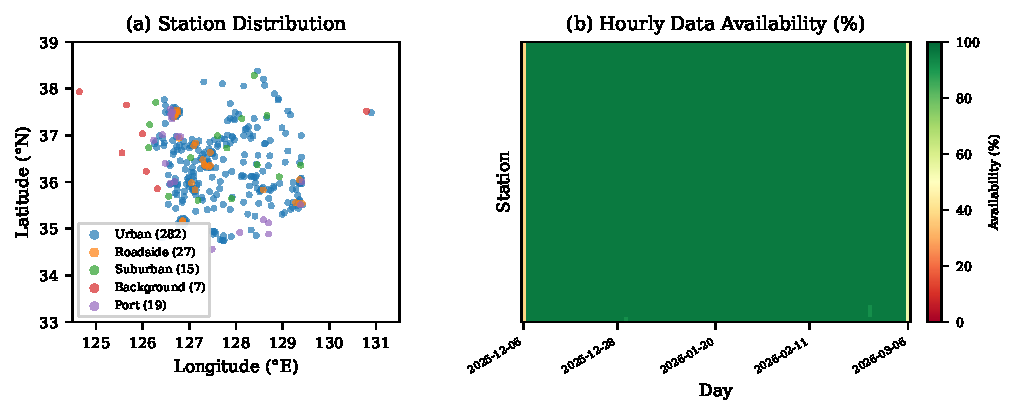
\includegraphics[width=\columnwidth]{figures/fig1_stations_availability.pdf}
\caption{(a)~Spatial distribution of 350 AirKorea stations by type. (b)~Percentage of stations experiencing data gaps exceeding 24~hours, by pollutant. Numbers above bars indicate total gap events across the network.}
\label{fig:stations}
\end{figure}

All six pollutants exhibit pronounced heteroscedasticity (figure~\ref{fig:noise}b). For PM\textsubscript{2.5}, the CV decreases from 0.379 at low concentrations (${\sim}4$~\si{\micro\gram/\meter\cubed}) to 0.035 at moderate levels (${\sim}14$~\si{\micro\gram/\meter\cubed}), then increases again to 0.258 at high levels (${\sim}57$~\si{\micro\gram/\meter\cubed}). This U-shaped relationship suggests that both detection-limit effects and source heterogeneity contribute to measurement uncertainty.

\begin{figure}[!t]
\centering
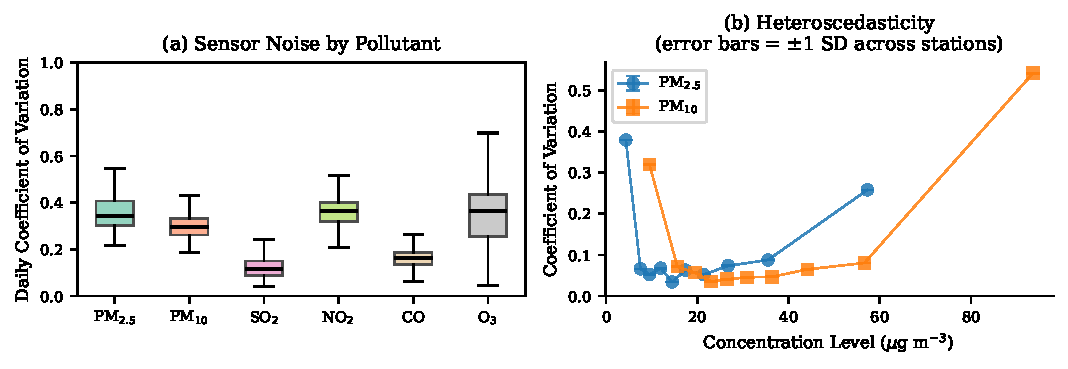
\includegraphics[width=\columnwidth]{figures/fig2_noise_analysis.pdf}
\caption{(a)~Distribution of daily CV across stations for each pollutant. (b)~Heteroscedasticity: CV as a function of concentration level for PM\textsubscript{2.5} and PM\textsubscript{10}.}
\label{fig:noise}
\end{figure}

\subsection{Sensor Drift}

Table~\ref{tab:drift} presents the drift analysis results. The fraction of stations exhibiting statistically significant drift ($p < 0.05$) varies from 25.3\% (PM\textsubscript{10}) to 61.3\% (SO\textsubscript{2}). Gaseous pollutants (SO\textsubscript{2}, CO, O\textsubscript{3}) show higher drift prevalence than particulate matter, which is consistent with the known sensitivity of electrochemical and optical gas analyzers to environmental conditions and reagent degradation.

\begin{table}[!t]
\centering
\caption{Drift Analysis Summary}
\label{tab:drift}
\begin{tabular}{lccc}
\toprule
\textbf{Pollutant} & \textbf{\% Sig. Drift} & \textbf{Median Rate} & \textbf{$|$Rate$|$ Median} \\
\midrule
PM\textsubscript{2.5} & 33.8\% & $-$0.43 & 1.01 \si{\micro\gram/\meter\cubed}/mo \\
PM\textsubscript{10}  & 25.3\% & $-$0.51 & 1.48 \si{\micro\gram/\meter\cubed}/mo \\
SO\textsubscript{2}   & 61.3\% & $-$0.06$\times 10^{-3}$ & 0.16$\times 10^{-3}$ ppm/mo \\
NO\textsubscript{2}   & 47.0\% & $-$0.50$\times 10^{-3}$ & 0.84$\times 10^{-3}$ ppm/mo \\
CO                     & 54.8\% & 9.6$\times 10^{-3}$ & 27.5$\times 10^{-3}$ ppm/mo \\
O\textsubscript{3}    & 44.8\% & 0.71$\times 10^{-3}$ & 1.29$\times 10^{-3}$ ppm/mo \\
\bottomrule
\end{tabular}
\end{table}

For PM\textsubscript{2.5}, the median drift rate among significantly drifting stations is $-0.43$~\si{\micro\gram/\meter\cubed}/month, suggesting a systematic negative bias that accumulates over time. Figure~\ref{fig:drift}a illustrates a representative drifting station where the 7-day rolling deviation from the regional mean shows a clear downward trend.

CUSUM analysis provides a complementary perspective: 72.2\% of PM\textsubscript{2.5} stations triggered a CUSUM alarm ($h = 10\hat{\sigma}$), substantially more than the 33.8\% identified by linear regression. This discrepancy arises because CUSUM detects \emph{transient} shifts that do not manifest as significant linear trends over the full period. Critically, CUSUM identifies \emph{when} drift begins: the median alarm occurs at day~18, indicating that most detectable drift emerges within the first three weeks---well within a standard quarterly calibration interval.

\begin{figure}[!t]
\centering
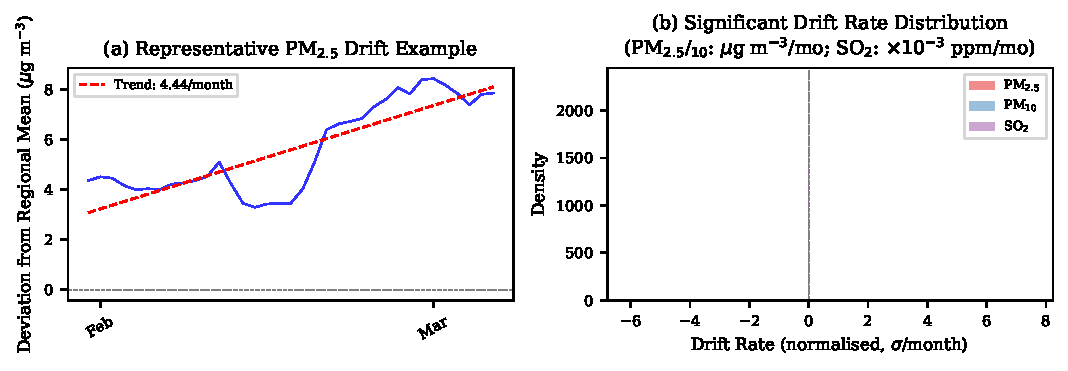
\includegraphics[width=\columnwidth]{figures/fig3_drift_analysis.pdf}
\caption{(a)~Drift example: 7-day rolling deviation from regional mean for a representative PM\textsubscript{2.5} station. (b)~Distribution of significant drift rates for PM\textsubscript{2.5}, PM\textsubscript{10}, and SO\textsubscript{2}.}
\label{fig:drift}
\end{figure}

\subsection{Spatial Cross-Calibration}

Among 279~co-located station pairs within 5~km, the median PM\textsubscript{2.5} Pearson correlation is 0.936 (figure~\ref{fig:crosscal}), indicating strong spatial coherence.

\begin{figure}[!t]
\centering
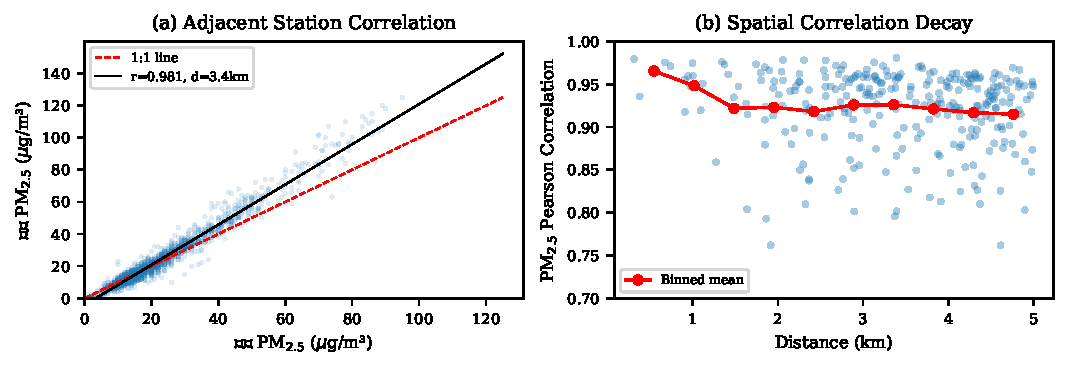
\includegraphics[width=\columnwidth]{figures/fig4_cross_calibration.pdf}
\caption{(a)~Scatter plot of PM\textsubscript{2.5} readings for the highest-correlation adjacent station pair. (b)~Spatial correlation decay: PM\textsubscript{2.5} correlation vs.\ inter-station distance for 279 pairs within 5~km.}
\label{fig:crosscal}
\end{figure}

However, the median RMSE of 6.94~\si{\micro\gram/\meter\cubed} and the finding that 23.7\% of pairs exhibit systematic biases ${>}5$~\si{\micro\gram/\meter\cubed} reveal non-trivial inter-station discrepancies.

Comparison with seven island background stations yields weaker correlations (median $r = 0.682$) due to spatial concentration gradients, with a median urban enhancement of 1.50~\si{\micro\gram/\meter\cubed}.

Among the 50 highest-correlation pairs, 26.0\% exhibit significant trends in inter-station bias ($p < 0.05$), indicating that even well-correlated stations develop diverging calibration states over three months.

\subsection{Measurement Uncertainty}

We estimate single-station PM\textsubscript{2.5} uncertainty by dividing pair-wise RMSE by $\sqrt{2}$, yielding $\pm$\SI{4.9}{\micro\gram/\meter\cubed} (median). This uncertainty is concentration-dependent: CV reaches 0.379 at low concentrations (${\sim}4$~\si{\micro\gram/\meter\cubed}), drops to 0.035 at moderate levels (${\sim}15$~\si{\micro\gram/\meter\cubed}), and rises to 0.258 at high levels (${\sim}57$~\si{\micro\gram/\meter\cubed}). The IQR of pair-wise RMSE [\num{5.42}, \num{8.79}]~\si{\micro\gram/\meter\cubed} indicates substantial precision variability. These estimates represent an upper bound on instrument uncertainty as they include micro-scale spatial variability.

\subsection{Station Reliability}

Overall data availability is high (97.4\% for urban PM\textsubscript{2.5}), but 36.3\% of stations experienced gaps exceeding 24~hours. MTBF varies by station type: roadside (394.2~days), urban (192.8~days), port (165.7~days), and suburban (65.7~days).

\subsection{Sensor Health Index}

Applying the proposed SHI to all 349~PM\textsubscript{2.5} stations (figure~\ref{fig:shi}) reveals that 78.5\% of stations are classified as Good (SHI~$\leq 0.2$), 18.1\% as Fair, 3.2\% as Poor, and 0.3\% (1~station) as Critical. The mean SHI is 0.158 (median = 0.141, SD = 0.090). The three component scores exhibit low inter-correlation (Drift--Noise: $r = 0.06$; Drift--Gap: $r = 0.27$; Noise--Gap: $r = 0.12$), confirming that the SHI captures complementary degradation modes. Suburban stations show the highest mean SHI (0.215), while roadside stations perform best (0.116), suggesting that maintenance schedules may need to account for station type.

\begin{figure}[!t]
\centering
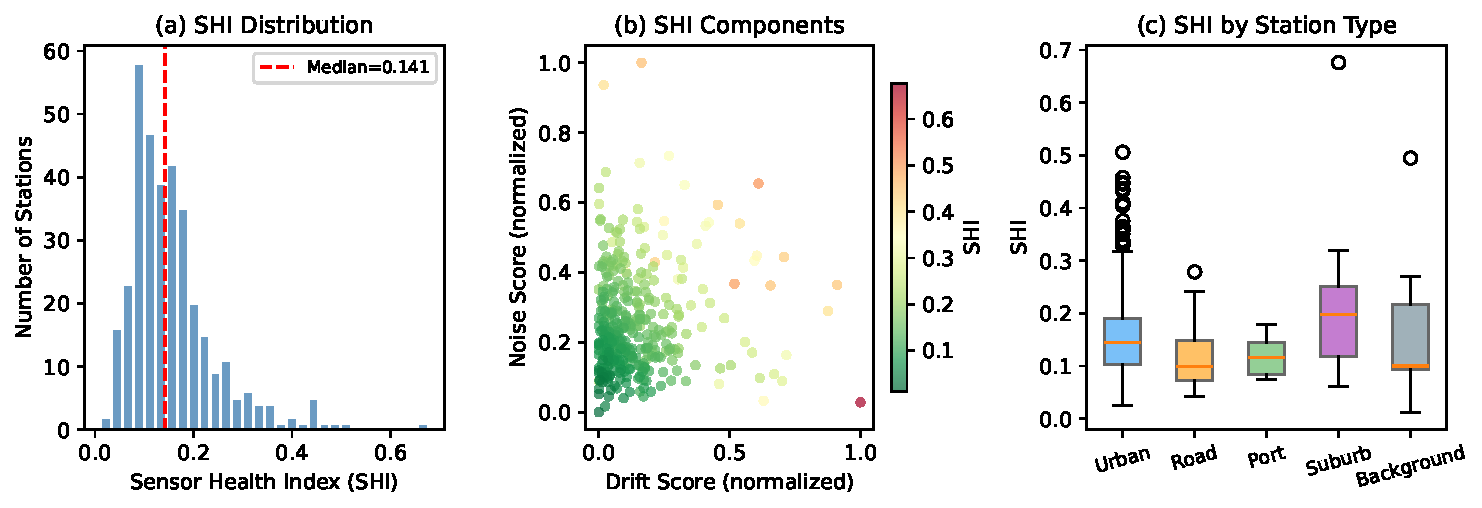
\includegraphics[width=\columnwidth]{figures/fig5_shi.pdf}
\caption{Sensor Health Index (SHI) analysis: (a)~distribution across 349 stations; (b)~component scores showing drift vs.\ noise with SHI as color; (c)~SHI distribution by station type.}
\label{fig:shi}
\end{figure}

\section{Discussion}

These findings have practical implications for network operation~\cite{epa2017qapp, duyzer2015representativeness}. Drift prevalence of 33.8--61.3\% over three months argues for monthly calibration verification, especially for gaseous analyzers ($>$45\% drift). The 23.7\% of pairs with biases ${>}5$~\si{\micro\gram/\meter\cubed} implies that data fusion should account for station-specific offsets~\cite{jiao2016cairsense}, and heteroscedastic noise requires concentration-dependent uncertainty quantification~\cite{schneider2017dqa}. The negative PM\textsubscript{2.5} drift ($-0.43$~\si{\micro\gram/\meter\cubed}/month) could yield ${\sim}1.3$~\si{\micro\gram/\meter\cubed} underestimation per quarter---non-negligible against Korea's 15~\si{\micro\gram/\meter\cubed} annual standard~\cite{kme2018standard}.

A potential concern is whether detected drift reflects instrument degradation or seasonal changes~\cite{miskell2018drift}. Three lines of evidence argue against a seasonal explanation: (1)~deviations from the regional mean remove the common seasonal signal; (2)~drift directions are heterogeneous within regions, inconsistent with systematic seasonal effects; (3)~inter-station drift residual correlation is near zero (median $r = -0.04$), confirming station-specific trends. These patterns are consistent with known degradation mechanisms in reference monitors, including filter clogging in BAM samplers and optical contamination in gas analyzers~\cite{shukla2022bam, heal2012particles}.

Limitations include the three-month observation window, which captures a single season and may not reflect annual patterns; the assumption that the regional mean is stable; and the 350-station subset representing approximately half the network. The proposed SHI uses equal component weighting as a baseline; optimal weighting should be determined through validation against maintenance records and expert assessment, which were unavailable for this study. Future work should extend to a full annual cycle, incorporate maintenance logs to validate drift detections, and develop automated flagging for real-time quality control~\cite{bai2020china, spinelle2017eufield}.

\section{Conclusion}

This paper provides the first systematic empirical characterization of in-field sensor performance across Korea's national air quality monitoring network, revealing widespread but heterogeneous drift, concentration-dependent noise, and non-trivial inter-station biases. We propose the Sensor Health Index (SHI), a composite metric integrating drift, noise, and availability that enables automated prioritization of maintenance resources. These empirical benchmarks and the SHI framework can inform calibration policies, data quality algorithms, and uncertainty propagation in air quality applications.

\section*{Data Availability}
Data used in this study were collected from the AirKorea Open API (\url{https://www.data.go.kr}) operated by the Korea Environment Corporation. The analysis code is available at \url{https://github.com/yjkim0123/airquality-sensor-characterization}.

\begin{thebibliography}{15}

\bibitem{kim2020airkorea}
Kim H, Kim H-J and Kim Y-H 2020 Review and evaluation of the national ambient air quality monitoring system in Korea \textit{J. Korean Soc. Atmos. Environ.} \textbf{36} 1--14

\bibitem{malings2020fine}
Malings C \textit{et al} 2020 Fine particle mass monitoring with low-cost sensors: Corrections and long-term performance evaluation \textit{Aerosol Sci. Technol.} \textbf{54} 160--174

\bibitem{zimmerman2018machine}
Zimmerman N \textit{et al} 2018 A machine learning calibration model using random forests to improve sensor performance for lower-cost air quality monitoring \textit{Atmos. Meas. Tech.} \textbf{11} 291--313

\bibitem{barkjohn2021development}
Barkjohn K K, Gantt B and Clements A L 2021 Development and application of a United States-wide correction for PM\textsubscript{2.5} data collected with the PurpleAir sensor \textit{Atmos. Meas. Tech.} \textbf{14} 4617--4637

\bibitem{munir2019analysing}
Munir S, Mayfield M, Coca D and Jubb S A 2019 Analysing the performance of low-cost air quality sensors, their drivers, relative benefits and calibration in cities---A case study in Sheffield \textit{Environ. Monit. Assess.} \textbf{191} 94

\bibitem{epa2017qapp}
U.S. Environmental Protection Agency 2017 Quality assurance handbook for air pollution measurement systems, Vol.~II: Ambient air quality monitoring program EPA-454/B-17-001

\bibitem{eu2008aqd}
European Parliament 2008 Directive 2008/50/EC on ambient air quality and cleaner air for Europe \textit{Off. J. Eur. Union} L~152 1--44

\bibitem{bai2020china}
Bai K \textit{et al} 2020 A homogenized daily in situ PM\textsubscript{2.5} concentration dataset from the national air quality monitoring network in China \textit{Earth Syst. Sci. Data} \textbf{12} 3067--3080

\bibitem{miskell2018drift}
Miskell G, Salmond J A and Williams D E 2018 Solution to the problem of calibration of low-cost air quality measurement sensors in networks \textit{ACS Sens.} \textbf{3} 832--843

\bibitem{jiao2016cairsense}
Jiao W \textit{et al} 2016 Community Air Sensor Network (CAIRSENSE) project: evaluation of low-cost sensor performance in a suburban environment in the southeastern United States \textit{Atmos. Meas. Tech.} \textbf{9} 5281--5292

\bibitem{schneider2017dqa}
Schneider P \textit{et al} 2017 Mapping urban air quality in near real-time using observations from low-cost sensors and model information \textit{Environ. Int.} \textbf{106} 234--247

\bibitem{kme2018standard}
Korea Ministry of Environment 2018 National ambient air quality standards (Enforcement Decree of the Clean Air Conservation Act) (Sejong, South Korea)

\bibitem{shukla2022bam}
Shukla K and Aggarwal S G 2022 A technical overview on beta-attenuation method for the monitoring of particulate matter in ambient air \textit{Aerosol Air Qual. Res.} \textbf{22} 220195

\bibitem{heal2012particles}
Heal M R, Kumar P and Harrison R M 2012 Particles, air quality, policy and health \textit{Chem. Soc. Rev.} \textbf{41} 6606--6630

\bibitem{duyzer2015representativeness}
Duyzer J, van den Hout D, Zandveld P and van Ratingen S 2015 Representativeness of air quality monitoring networks \textit{Atmos. Environ.} \textbf{104} 88--101

\bibitem{spinelle2017eufield}
Spinelle L, Gerboles M, Villani M G, Aleixandre M and Bonavitacola F 2017 Field calibration of a cluster of low-cost commercially available sensors for air quality monitoring. Part~B: NO, CO and CO\textsubscript{2} \textit{Sens. Actuators B Chem.} \textbf{238} 706--715

\bibitem{page1954cusum}
Page E S 1954 Continuous inspection schemes \textit{Biometrika} \textbf{41} 100--115

\end{thebibliography}

\end{document}
